\documentclass[1p]{elsarticle_modified}
%\bibliographystyle{elsarticle-num}

%\usepackage[colorlinks]{hyperref}
%\usepackage{abbrmath_seonhwa} %\Abb, \Ascr, \Acal ,\Abf, \Afrak
\usepackage{amsfonts}
\usepackage{amssymb}
\usepackage{amsmath}
\usepackage{amsthm}
\usepackage{scalefnt}
\usepackage{amsbsy}
\usepackage{kotex}
\usepackage{caption}
\usepackage{subfig}
\usepackage{color}
\usepackage{graphicx}
\usepackage{xcolor} %% white, black, red, green, blue, cyan, magenta, yellow
\usepackage{float}
\usepackage{setspace}
\usepackage{hyperref}

\usepackage{tikz}
\usetikzlibrary{arrows}

\usepackage{multirow}
\usepackage{array} % fixed length table
\usepackage{hhline}

%%%%%%%%%%%%%%%%%%%%%
\makeatletter
\renewcommand*\env@matrix[1][\arraystretch]{%
	\edef\arraystretch{#1}%
	\hskip -\arraycolsep
	\let\@ifnextchar\new@ifnextchar
	\array{*\c@MaxMatrixCols c}}
\makeatother %https://tex.stackexchange.com/questions/14071/how-can-i-increase-the-line-spacing-in-a-matrix
%%%%%%%%%%%%%%%

\usepackage[normalem]{ulem}

\newcommand{\msout}[1]{\ifmmode\text{\sout{\ensuremath{#1}}}\else\sout{#1}\fi}
%SOURCE: \msout is \stkout macro in https://tex.stackexchange.com/questions/20609/strikeout-in-math-mode

\newcommand{\cancel}[1]{
	\ifmmode
	{\color{red}\msout{#1}}
	\else
	{\color{red}\sout{#1}}
	\fi
}

\newcommand{\add}[1]{
	{\color{blue}\uwave{#1}}
}

\newcommand{\replace}[2]{
	\ifmmode
	{\color{red}\msout{#1}}{\color{blue}\uwave{#2}}
	\else
	{\color{red}\sout{#1}}{\color{blue}\uwave{#2}}
	\fi
}

\newcommand{\Sol}{\mathcal{S}} %segment
\newcommand{\D}{D} %diagram
\newcommand{\A}{\mathcal{A}} %arc


%%%%%%%%%%%%%%%%%%%%%%%%%%%%%5 test

\def\sl{\operatorname{\textup{SL}}(2,\Cbb)}
\def\psl{\operatorname{\textup{PSL}}(2,\Cbb)}
\def\quan{\mkern 1mu \triangleright \mkern 1mu}

\theoremstyle{definition}
\newtheorem{thm}{Theorem}[section]
\newtheorem{prop}[thm]{Proposition}
\newtheorem{lem}[thm]{Lemma}
\newtheorem{ques}[thm]{Question}
\newtheorem{cor}[thm]{Corollary}
\newtheorem{defn}[thm]{Definition}
\newtheorem{exam}[thm]{Example}
\newtheorem{rmk}[thm]{Remark}
\newtheorem{alg}[thm]{Algorithm}

\newcommand{\I}{\sqrt{-1}}
\begin{document}

%\begin{frontmatter}
%
%\title{Boundary parabolic representations of knots up to 8 crossings}
%
%%% Group authors per affiliation:
%\author{Yunhi Cho} 
%\address{Department of Mathematics, University of Seoul, Seoul, Korea}
%\ead{yhcho@uos.ac.kr}
%
%
%\author{Seonhwa Kim} %\fnref{s_kim}}
%\address{Center for Geometry and Physics, Institute for Basic Science, Pohang, 37673, Korea}
%\ead{ryeona17@ibs.re.kr}
%
%\author{Hyuk Kim}
%\address{Department of Mathematical Sciences, Seoul National University, Seoul 08826, Korea}
%\ead{hyukkim@snu.ac.kr}
%
%\author{Seokbeom Yoon}
%\address{Department of Mathematical Sciences, Seoul National University, Seoul, 08826,  Korea}
%\ead{sbyoon15@snu.ac.kr}
%
%\begin{abstract}
%We find all boundary parabolic representation of knots up to 8 crossings.
%
%\end{abstract}
%\begin{keyword}
%    \MSC[2010] 57M25 
%\end{keyword}
%
%\end{frontmatter}

%\linenumbers
%\tableofcontents
%
\newcommand\colored[1]{\textcolor{white}{\rule[-0.35ex]{0.8em}{1.4ex}}\kern-0.8em\color{red} #1}%
%\newcommand\colored[1]{\textcolor{white}{ #1}\kern-2.17ex	\textcolor{white}{ #1}\kern-1.81ex	\textcolor{white}{ #1}\kern-2.15ex\color{red}#1	}

{\Large $\underline{12a_{0187}~(K12a_{0187})}$}

\setlength{\tabcolsep}{10pt}
\renewcommand{\arraystretch}{1.6}
\vspace{1cm}\begin{tabular}{m{100pt}>{\centering\arraybackslash}m{274pt}}
\multirow{5}{120pt}{
	\centering
	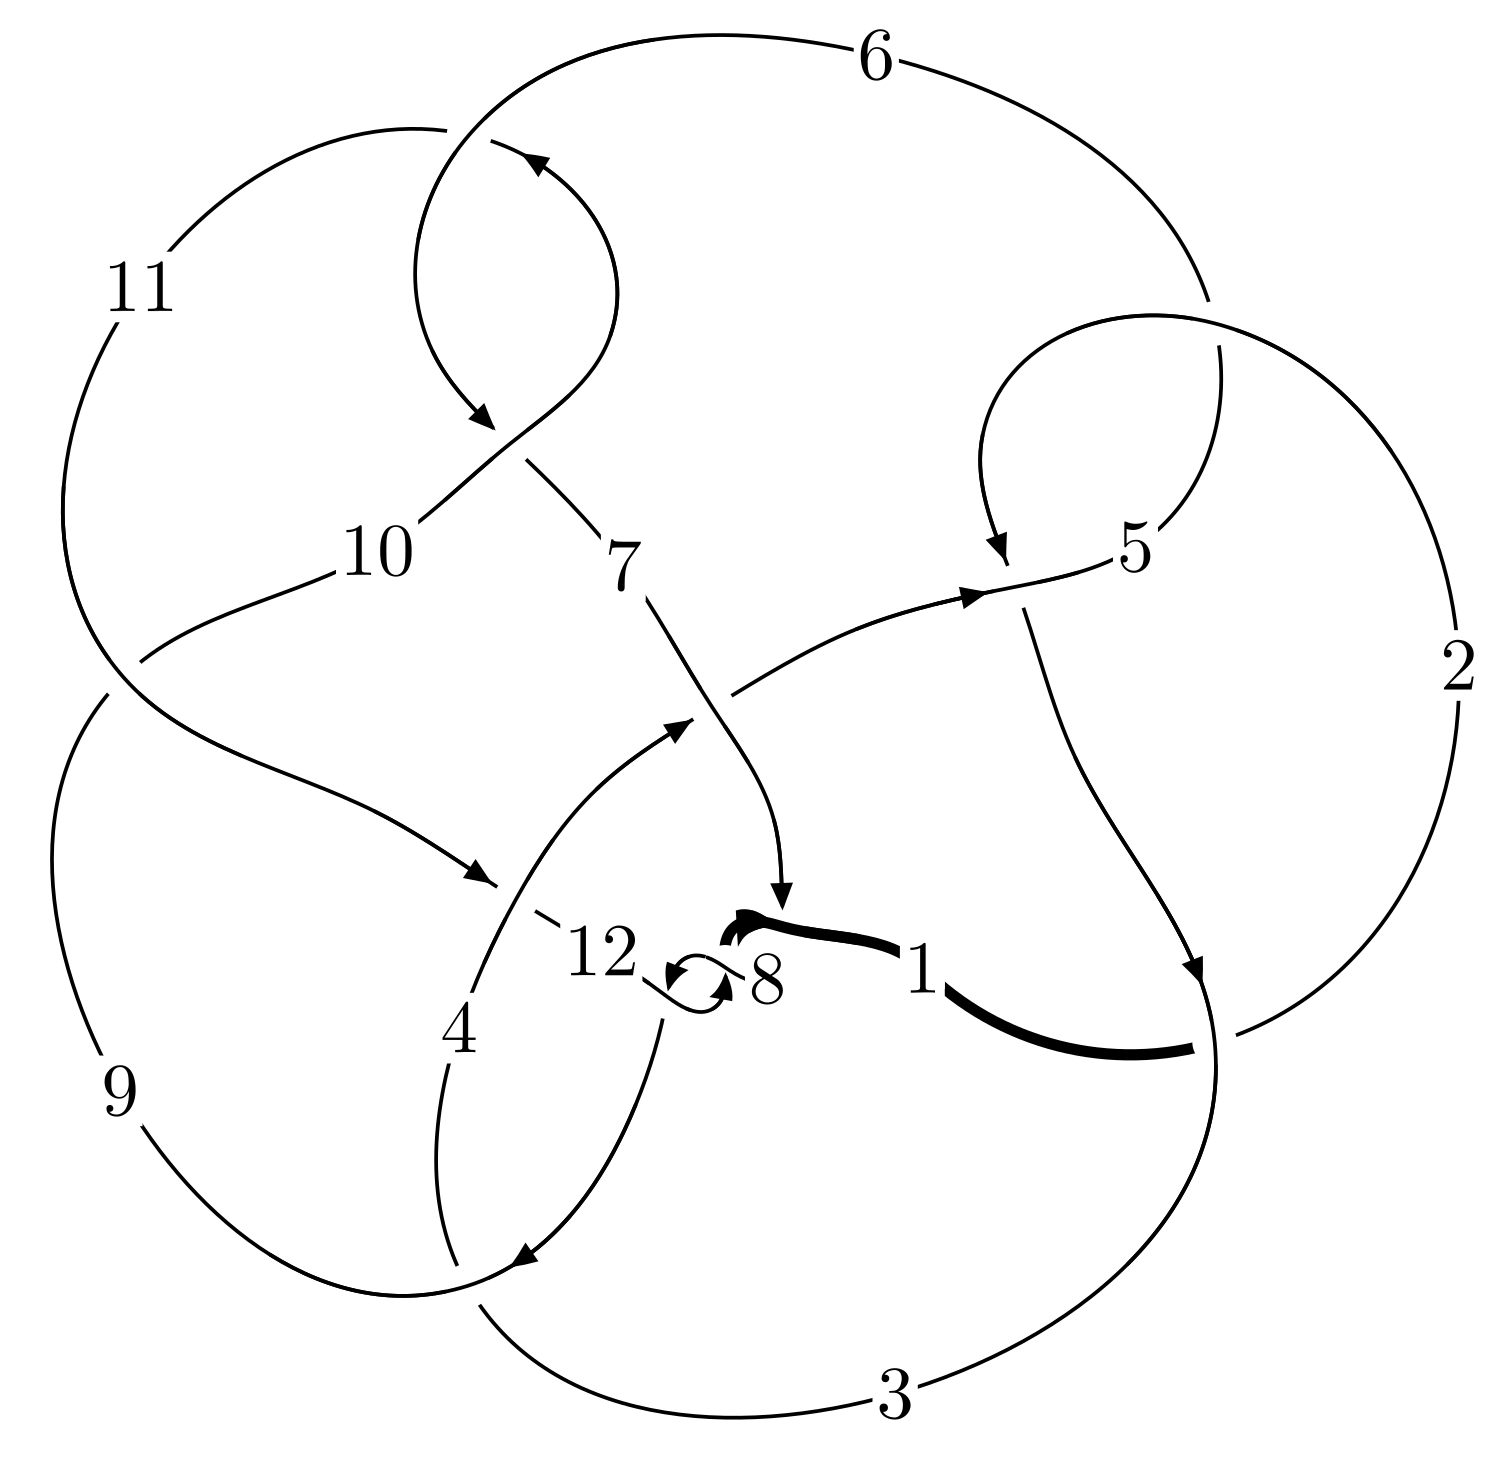
\includegraphics[width=112pt]{../../../GIT/diagram.site/Diagrams/png/988_12a_0187.png}\\
\ \ \ A knot diagram\footnotemark}&
\allowdisplaybreaks
\textbf{Linearized knot diagam} \\
\cline{2-2}
 &
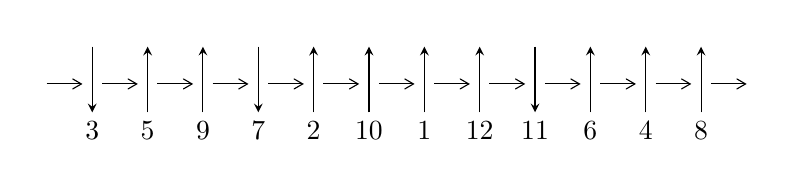
\begin{tikzpicture}[x=20pt, y=17pt]
	% nodes
	\node (C0) at (0, 0) {};
	\node (C1) at (1, 0) {};
	\node (C1U) at (1, +1) {};
	\node (C1D) at (1, -1) {3};

	\node (C2) at (2, 0) {};
	\node (C2U) at (2, +1) {};
	\node (C2D) at (2, -1) {5};

	\node (C3) at (3, 0) {};
	\node (C3U) at (3, +1) {};
	\node (C3D) at (3, -1) {9};

	\node (C4) at (4, 0) {};
	\node (C4U) at (4, +1) {};
	\node (C4D) at (4, -1) {7};

	\node (C5) at (5, 0) {};
	\node (C5U) at (5, +1) {};
	\node (C5D) at (5, -1) {2};

	\node (C6) at (6, 0) {};
	\node (C6U) at (6, +1) {};
	\node (C6D) at (6, -1) {10};

	\node (C7) at (7, 0) {};
	\node (C7U) at (7, +1) {};
	\node (C7D) at (7, -1) {1};

	\node (C8) at (8, 0) {};
	\node (C8U) at (8, +1) {};
	\node (C8D) at (8, -1) {12};

	\node (C9) at (9, 0) {};
	\node (C9U) at (9, +1) {};
	\node (C9D) at (9, -1) {11};

	\node (C10) at (10, 0) {};
	\node (C10U) at (10, +1) {};
	\node (C10D) at (10, -1) {6};

	\node (C11) at (11, 0) {};
	\node (C11U) at (11, +1) {};
	\node (C11D) at (11, -1) {4};

	\node (C12) at (12, 0) {};
	\node (C12U) at (12, +1) {};
	\node (C12D) at (12, -1) {8};
	\node (C13) at (13, 0) {};

	% arrows
	\draw[->,>={angle 60}]
	(C0) edge (C1) (C1) edge (C2) (C2) edge (C3) (C3) edge (C4) (C4) edge (C5) (C5) edge (C6) (C6) edge (C7) (C7) edge (C8) (C8) edge (C9) (C9) edge (C10) (C10) edge (C11) (C11) edge (C12) (C12) edge (C13) ;	\draw[->,>=stealth]
	(C1U) edge (C1D) (C2D) edge (C2U) (C3D) edge (C3U) (C4U) edge (C4D) (C5D) edge (C5U) (C6D) edge (C6U) (C7D) edge (C7U) (C8D) edge (C8U) (C9U) edge (C9D) (C10D) edge (C10U) (C11D) edge (C11U) (C12D) edge (C12U) ;
	\end{tikzpicture} \\
\hhline{~~} \\& 
\textbf{Solving Sequence} \\ \cline{2-2} 
 &
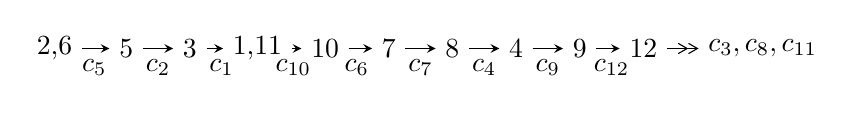
\begin{tikzpicture}[x=23pt, y=7pt]
	% node
	\node (A0) at (-1/8, 0) {2,6};
	\node (A1) at (1, 0) {5};
	\node (A2) at (2, 0) {3};
	\node (A3) at (49/16, 0) {1,11};
	\node (A4) at (33/8, 0) {10};
	\node (A5) at (41/8, 0) {7};
	\node (A6) at (49/8, 0) {8};
	\node (A7) at (57/8, 0) {4};
	\node (A8) at (65/8, 0) {9};
	\node (A9) at (73/8, 0) {12};
	\node (C1) at (1/2, -1) {$c_{5}$};
	\node (C2) at (3/2, -1) {$c_{2}$};
	\node (C3) at (5/2, -1) {$c_{1}$};
	\node (C4) at (29/8, -1) {$c_{10}$};
	\node (C5) at (37/8, -1) {$c_{6}$};
	\node (C6) at (45/8, -1) {$c_{7}$};
	\node (C7) at (53/8, -1) {$c_{4}$};
	\node (C8) at (61/8, -1) {$c_{9}$};
	\node (C9) at (69/8, -1) {$c_{12}$};
	\node (A10) at (11, 0) {$c_{3},c_{8},c_{11}$};

	% edge
	\draw[->,>=stealth]	
	(A0) edge (A1) (A1) edge (A2) (A2) edge (A3) (A3) edge (A4) (A4) edge (A5) (A5) edge (A6) (A6) edge (A7) (A7) edge (A8) (A8) edge (A9) ;
	\draw[->>,>={angle 60}]	
	(A9) edge (A10);
\end{tikzpicture} \\ 

\end{tabular} \\

\footnotetext{
The image of knot diagram is generated by the software ``\textbf{Draw programme}" developed by Andrew Bartholomew(\url{http://www.layer8.co.uk/maths/draw/index.htm\#Running-draw}), where we modified some parts for our purpose(\url{https://github.com/CATsTAILs/LinksPainter}).
}\phantom \\ \newline 
\centering \textbf{Ideals for irreducible components\footnotemark of $X_{\text{par}}$} 
 
\begin{align*}
I^u_{1}&=\langle 
-4.70828\times10^{211} u^{102}-4.30580\times10^{211} u^{101}+\cdots+2.02673\times10^{212} b-2.48946\times10^{212},\\
\phantom{I^u_{1}}&\phantom{= \langle  }4.27526\times10^{212} u^{102}+1.62447\times10^{213} u^{101}+\cdots+1.82405\times10^{213} a-3.78144\times10^{212},\\
\phantom{I^u_{1}}&\phantom{= \langle  }u^{103}+2 u^{102}+\cdots-50 u-9\rangle \\
I^u_{2}&=\langle 
b+1,\;3 a-3 u+4,\;u^2- u+1\rangle \\
\\
\end{align*}
\raggedright * 2 irreducible components of $\dim_{\mathbb{C}}=0$, with total 105 representations.\\
\footnotetext{All coefficients of polynomials are rational numbers. But the coefficients are sometimes approximated in decimal forms when there is not enough margin.}
\newpage
\renewcommand{\arraystretch}{1}
\centering \section*{I. $I^u_{1}= \langle -4.71\times10^{211} u^{102}-4.31\times10^{211} u^{101}+\cdots+2.03\times10^{212} b-2.49\times10^{212},\;4.28\times10^{212} u^{102}+1.62\times10^{213} u^{101}+\cdots+1.82\times10^{213} a-3.78\times10^{212},\;u^{103}+2 u^{102}+\cdots-50 u-9 \rangle$}
\flushleft \textbf{(i) Arc colorings}\\
\begin{tabular}{m{7pt} m{180pt} m{7pt} m{180pt} }
\flushright $a_{2}=$&$\begin{pmatrix}0\\u\end{pmatrix}$ \\
\flushright $a_{6}=$&$\begin{pmatrix}1\\0\end{pmatrix}$ \\
\flushright $a_{5}=$&$\begin{pmatrix}1\\u^2\end{pmatrix}$ \\
\flushright $a_{3}=$&$\begin{pmatrix}u\\u^3+u\end{pmatrix}$ \\
\flushright $a_{1}=$&$\begin{pmatrix}u^3\\u^5+u^3+u\end{pmatrix}$ \\
\flushright $a_{11}=$&$\begin{pmatrix}-0.234382 u^{102}-0.890582 u^{101}+\cdots+27.2644 u+0.207310\\0.232309 u^{102}+0.212451 u^{101}+\cdots+5.06954 u+1.22831\end{pmatrix}$ \\
\flushright $a_{10}=$&$\begin{pmatrix}-0.466692 u^{102}-1.10303 u^{101}+\cdots+22.1949 u-1.02100\\0.232309 u^{102}+0.212451 u^{101}+\cdots+5.06954 u+1.22831\end{pmatrix}$ \\
\flushright $a_{7}=$&$\begin{pmatrix}-0.267327 u^{102}-0.877958 u^{101}+\cdots+39.1849 u+7.35328\\0.374555 u^{102}+0.677940 u^{101}+\cdots-9.16517 u-0.221474\end{pmatrix}$ \\
\flushright $a_{8}=$&$\begin{pmatrix}0.237025 u^{102}+0.234288 u^{101}+\cdots+15.8996 u+3.19729\\0.115727 u^{102}+0.335221 u^{101}+\cdots-7.46104 u-0.621629\end{pmatrix}$ \\
\flushright $a_{4}=$&$\begin{pmatrix}0.150719 u^{102}-0.268946 u^{101}+\cdots+12.7692 u+8.10850\\0.538052 u^{102}+0.982186 u^{101}+\cdots-20.4638 u-3.33616\end{pmatrix}$ \\
\flushright $a_{9}=$&$\begin{pmatrix}-0.243327 u^{102}-0.831816 u^{101}+\cdots+38.7154 u+9.33905\\0.344667 u^{102}+0.390802 u^{101}+\cdots+1.82827 u+2.29816\end{pmatrix}$ \\
\flushright $a_{12}=$&$\begin{pmatrix}-0.238737 u^{102}-1.06579 u^{101}+\cdots+25.5129 u-2.83305\\0.272415 u^{102}+0.179279 u^{101}+\cdots+8.93923 u+1.31134\end{pmatrix}$\\&\end{tabular}
\flushleft \textbf{(ii) Obstruction class $= -1$}\\~\\
\flushleft \textbf{(iii) Cusp Shapes $= 1.09329 u^{102}+1.70936 u^{101}+\cdots-12.5511 u-1.22773$}\\~\\
\newpage\renewcommand{\arraystretch}{1}
\flushleft \textbf{(iv) u-Polynomials at the component}\newline \\
\begin{tabular}{m{50pt}|m{274pt}}
Crossings & \hspace{64pt}u-Polynomials at each crossing \\
\hline $$\begin{aligned}c_{1}\end{aligned}$$&$\begin{aligned}
&u^{103}+44 u^{102}+\cdots+1510 u-81
\end{aligned}$\\
\hline $$\begin{aligned}c_{2},c_{5}\end{aligned}$$&$\begin{aligned}
&u^{103}+2 u^{102}+\cdots-50 u-9
\end{aligned}$\\
\hline $$\begin{aligned}c_{3}\end{aligned}$$&$\begin{aligned}
&9(9 u^{103}-132 u^{102}+\cdots+8034 u-2563)
\end{aligned}$\\
\hline $$\begin{aligned}c_{4}\end{aligned}$$&$\begin{aligned}
&9(9 u^{103}+87 u^{102}+\cdots-19058 u-1196)
\end{aligned}$\\
\hline $$\begin{aligned}c_{6},c_{10}\end{aligned}$$&$\begin{aligned}
&u^{103}-3 u^{102}+\cdots+3 u-1
\end{aligned}$\\
\hline $$\begin{aligned}c_{7},c_{8},c_{12}\end{aligned}$$&$\begin{aligned}
&u^{103}+3 u^{102}+\cdots-3 u-1
\end{aligned}$\\
\hline $$\begin{aligned}c_{9}\end{aligned}$$&$\begin{aligned}
&u^{103}+37 u^{102}+\cdots+13 u-1
\end{aligned}$\\
\hline $$\begin{aligned}c_{11}\end{aligned}$$&$\begin{aligned}
&u^{103}-5 u^{102}+\cdots+648 u-108
\end{aligned}$\\
\hline
\end{tabular}\\~\\
\newpage\renewcommand{\arraystretch}{1}
\flushleft \textbf{(v) Riley Polynomials at the component}\newline \\
\begin{tabular}{m{50pt}|m{274pt}}
Crossings & \hspace{64pt}Riley Polynomials at each crossing \\
\hline $$\begin{aligned}c_{1}\end{aligned}$$&$\begin{aligned}
&y^{103}+32 y^{102}+\cdots+1346818 y-6561
\end{aligned}$\\
\hline $$\begin{aligned}c_{2},c_{5}\end{aligned}$$&$\begin{aligned}
&y^{103}+44 y^{102}+\cdots+1510 y-81
\end{aligned}$\\
\hline $$\begin{aligned}c_{3}\end{aligned}$$&$\begin{aligned}
&81(81 y^{103}+11916 y^{102}+\cdots+1.84130\times10^{8} y-6568969)
\end{aligned}$\\
\hline $$\begin{aligned}c_{4}\end{aligned}$$&$\begin{aligned}
&81(81 y^{103}+11295 y^{102}+\cdots+1.43926\times10^{8} y-1430416)
\end{aligned}$\\
\hline $$\begin{aligned}c_{6},c_{10}\end{aligned}$$&$\begin{aligned}
&y^{103}+37 y^{102}+\cdots+13 y-1
\end{aligned}$\\
\hline $$\begin{aligned}c_{7},c_{8},c_{12}\end{aligned}$$&$\begin{aligned}
&y^{103}+97 y^{102}+\cdots+13 y-1
\end{aligned}$\\
\hline $$\begin{aligned}c_{9}\end{aligned}$$&$\begin{aligned}
&y^{103}+45 y^{102}+\cdots-379 y-1
\end{aligned}$\\
\hline $$\begin{aligned}c_{11}\end{aligned}$$&$\begin{aligned}
&y^{103}+15 y^{102}+\cdots-153576 y-11664
\end{aligned}$\\
\hline
\end{tabular}\\~\\
\newpage\flushleft \textbf{(vi) Complex Volumes and Cusp Shapes}
$$\begin{array}{c|c|c}  
\text{Solutions to }I^u_{1}& \I (\text{vol} + \sqrt{-1}CS) & \text{Cusp shape}\\
 \hline 
\begin{aligned}
u &= -0.871098 + 0.491257 I \\
a &= -1.30022 - 0.63958 I \\
b &= -0.694924 - 1.068860 I\end{aligned}
 & \phantom{-}2.78356 + 8.56668 I & \phantom{-0.000000 } 0 \\ \hline\begin{aligned}
u &= -0.871098 - 0.491257 I \\
a &= -1.30022 + 0.63958 I \\
b &= -0.694924 + 1.068860 I\end{aligned}
 & \phantom{-}2.78356 - 8.56668 I & \phantom{-0.000000 } 0 \\ \hline\begin{aligned}
u &= \phantom{-}0.481345 + 0.878527 I \\
a &= -8.55020 - 1.64997 I \\
b &= -0.531227 + 0.886277 I\end{aligned}
 & -5.02226 + 0.00767 I & \phantom{-0.000000 } 0 \\ \hline\begin{aligned}
u &= \phantom{-}0.481345 - 0.878527 I \\
a &= -8.55020 + 1.64997 I \\
b &= -0.531227 - 0.886277 I\end{aligned}
 & -5.02226 - 0.00767 I & \phantom{-0.000000 } 0 \\ \hline\begin{aligned}
u &= \phantom{-}0.915500 + 0.391024 I \\
a &= -1.287160 + 0.339540 I \\
b &= -0.626849 + 0.812428 I\end{aligned}
 & \phantom{-}3.16321 - 0.76735 I & \phantom{-0.000000 } 0 \\ \hline\begin{aligned}
u &= \phantom{-}0.915500 - 0.391024 I \\
a &= -1.287160 - 0.339540 I \\
b &= -0.626849 - 0.812428 I\end{aligned}
 & \phantom{-}3.16321 + 0.76735 I & \phantom{-0.000000 } 0 \\ \hline\begin{aligned}
u &= \phantom{-}0.111367 + 0.987800 I \\
a &= -0.314049 - 0.426026 I \\
b &= -0.557089 + 0.278730 I\end{aligned}
 & -1.61354 + 2.06379 I & \phantom{-0.000000 } 0 \\ \hline\begin{aligned}
u &= \phantom{-}0.111367 - 0.987800 I \\
a &= -0.314049 + 0.426026 I \\
b &= -0.557089 - 0.278730 I\end{aligned}
 & -1.61354 - 2.06379 I & \phantom{-0.000000 } 0 \\ \hline\begin{aligned}
u &= \phantom{-}0.590356 + 0.821048 I \\
a &= \phantom{-}1.35154 - 2.18344 I \\
b &= \phantom{-}0.555019 - 0.805027 I\end{aligned}
 & \phantom{-}0.597431 + 0.086793 I & \phantom{-0.000000 } 0 \\ \hline\begin{aligned}
u &= \phantom{-}0.590356 - 0.821048 I \\
a &= \phantom{-}1.35154 + 2.18344 I \\
b &= \phantom{-}0.555019 + 0.805027 I\end{aligned}
 & \phantom{-}0.597431 - 0.086793 I & \phantom{-0.000000 } 0\\
 \hline 
 \end{array}$$\newpage$$\begin{array}{c|c|c}  
\text{Solutions to }I^u_{1}& \I (\text{vol} + \sqrt{-1}CS) & \text{Cusp shape}\\
 \hline 
\begin{aligned}
u &= -0.453314 + 0.866625 I \\
a &= \phantom{-}1.014640 + 0.981164 I \\
b &= \phantom{-}1.155570 - 0.097756 I\end{aligned}
 & \phantom{-}1.47294 - 1.87526 I & \phantom{-0.000000 } 0 \\ \hline\begin{aligned}
u &= -0.453314 - 0.866625 I \\
a &= \phantom{-}1.014640 - 0.981164 I \\
b &= \phantom{-}1.155570 + 0.097756 I\end{aligned}
 & \phantom{-}1.47294 + 1.87526 I & \phantom{-0.000000 } 0 \\ \hline\begin{aligned}
u &= \phantom{-}0.569820 + 0.848750 I \\
a &= -0.214973 + 0.102311 I \\
b &= \phantom{-}0.197507 + 0.130121 I\end{aligned}
 & \phantom{-}0.45171 + 2.26396 I & \phantom{-0.000000 } 0 \\ \hline\begin{aligned}
u &= \phantom{-}0.569820 - 0.848750 I \\
a &= -0.214973 - 0.102311 I \\
b &= \phantom{-}0.197507 - 0.130121 I\end{aligned}
 & \phantom{-}0.45171 - 2.26396 I & \phantom{-0.000000 } 0 \\ \hline\begin{aligned}
u &= \phantom{-}0.359432 + 0.905150 I \\
a &= -0.75669 + 1.89295 I \\
b &= \phantom{-}0.352860 - 0.854813 I\end{aligned}
 & -0.888701 + 0.166715 I & \phantom{-0.000000 } 0 \\ \hline\begin{aligned}
u &= \phantom{-}0.359432 - 0.905150 I \\
a &= -0.75669 - 1.89295 I \\
b &= \phantom{-}0.352860 + 0.854813 I\end{aligned}
 & -0.888701 - 0.166715 I & \phantom{-0.000000 } 0 \\ \hline\begin{aligned}
u &= -0.921960 + 0.458261 I \\
a &= \phantom{-}1.47257 - 0.41314 I \\
b &= \phantom{-}0.852313 - 0.561544 I\end{aligned}
 & -1.90097 + 6.60861 I & \phantom{-0.000000 } 0 \\ \hline\begin{aligned}
u &= -0.921960 - 0.458261 I \\
a &= \phantom{-}1.47257 + 0.41314 I \\
b &= \phantom{-}0.852313 + 0.561544 I\end{aligned}
 & -1.90097 - 6.60861 I & \phantom{-0.000000 } 0 \\ \hline\begin{aligned}
u &= -0.793954 + 0.554908 I \\
a &= -1.60966 + 0.27728 I \\
b &= -0.864736 + 0.590779 I\end{aligned}
 & \phantom{-}4.25085 + 2.77419 I & \phantom{-0.000000 } 0 \\ \hline\begin{aligned}
u &= -0.793954 - 0.554908 I \\
a &= -1.60966 - 0.27728 I \\
b &= -0.864736 - 0.590779 I\end{aligned}
 & \phantom{-}4.25085 - 2.77419 I & \phantom{-0.000000 } 0\\
 \hline 
 \end{array}$$\newpage$$\begin{array}{c|c|c}  
\text{Solutions to }I^u_{1}& \I (\text{vol} + \sqrt{-1}CS) & \text{Cusp shape}\\
 \hline 
\begin{aligned}
u &= \phantom{-}0.495018 + 0.831311 I \\
a &= \phantom{-}2.68722 + 5.91244 I \\
b &= -0.462208 - 0.898317 I\end{aligned}
 & -4.88019 + 3.96585 I & \phantom{-0.000000 } 0 \\ \hline\begin{aligned}
u &= \phantom{-}0.495018 - 0.831311 I \\
a &= \phantom{-}2.68722 - 5.91244 I \\
b &= -0.462208 + 0.898317 I\end{aligned}
 & -4.88019 - 3.96585 I & \phantom{-0.000000 } 0 \\ \hline\begin{aligned}
u &= -0.293989 + 0.900677 I \\
a &= -0.340712 - 1.361400 I \\
b &= -0.846553 - 0.778278 I\end{aligned}
 & -6.38836 + 1.72239 I & \phantom{-0.000000 } 0 \\ \hline\begin{aligned}
u &= -0.293989 - 0.900677 I \\
a &= -0.340712 + 1.361400 I \\
b &= -0.846553 + 0.778278 I\end{aligned}
 & -6.38836 - 1.72239 I & \phantom{-0.000000 } 0 \\ \hline\begin{aligned}
u &= -0.277077 + 1.032330 I \\
a &= -1.19938 - 1.04039 I \\
b &= -0.201061 + 1.183910 I\end{aligned}
 & -5.76408 - 0.70494 I & \phantom{-0.000000 } 0 \\ \hline\begin{aligned}
u &= -0.277077 - 1.032330 I \\
a &= -1.19938 + 1.04039 I \\
b &= -0.201061 - 1.183910 I\end{aligned}
 & -5.76408 + 0.70494 I & \phantom{-0.000000 } 0 \\ \hline\begin{aligned}
u &= -0.986142 + 0.425293 I \\
a &= \phantom{-}1.39902 + 0.48943 I \\
b &= \phantom{-}0.684015 + 1.076400 I\end{aligned}
 & -3.46407 + 12.32820 I & \phantom{-0.000000 } 0 \\ \hline\begin{aligned}
u &= -0.986142 - 0.425293 I \\
a &= \phantom{-}1.39902 - 0.48943 I \\
b &= \phantom{-}0.684015 - 1.076400 I\end{aligned}
 & -3.46407 - 12.32820 I & \phantom{-0.000000 } 0 \\ \hline\begin{aligned}
u &= -0.610418 + 0.687254 I \\
a &= \phantom{-}1.81549 + 0.03994 I \\
b &= \phantom{-}0.914625 - 0.659767 I\end{aligned}
 & \phantom{-}3.31217 - 2.28195 I & \phantom{-0.000000 } 0 \\ \hline\begin{aligned}
u &= -0.610418 - 0.687254 I \\
a &= \phantom{-}1.81549 - 0.03994 I \\
b &= \phantom{-}0.914625 + 0.659767 I\end{aligned}
 & \phantom{-}3.31217 + 2.28195 I & \phantom{-0.000000 } 0\\
 \hline 
 \end{array}$$\newpage$$\begin{array}{c|c|c}  
\text{Solutions to }I^u_{1}& \I (\text{vol} + \sqrt{-1}CS) & \text{Cusp shape}\\
 \hline 
\begin{aligned}
u &= -0.429365 + 0.993415 I \\
a &= -2.23623 - 0.66942 I \\
b &= -0.793940 + 1.063610 I\end{aligned}
 & -7.22938 - 4.55942 I & \phantom{-0.000000 } 0 \\ \hline\begin{aligned}
u &= -0.429365 - 0.993415 I \\
a &= -2.23623 + 0.66942 I \\
b &= -0.793940 - 1.063610 I\end{aligned}
 & -7.22938 + 4.55942 I & \phantom{-0.000000 } 0 \\ \hline\begin{aligned}
u &= \phantom{-}0.575604 + 0.917006 I \\
a &= \phantom{-}3.51154 - 0.47561 I \\
b &= \phantom{-}0.558359 + 0.901843 I\end{aligned}
 & \phantom{-}0.28262 + 4.54488 I & \phantom{-0.000000 } 0 \\ \hline\begin{aligned}
u &= \phantom{-}0.575604 - 0.917006 I \\
a &= \phantom{-}3.51154 + 0.47561 I \\
b &= \phantom{-}0.558359 - 0.901843 I\end{aligned}
 & \phantom{-}0.28262 - 4.54488 I & \phantom{-0.000000 } 0 \\ \hline\begin{aligned}
u &= -0.145915 + 0.904009 I \\
a &= -0.387490 - 0.748969 I \\
b &= \phantom{-}0.477410 + 1.112370 I\end{aligned}
 & -2.20452 + 2.91537 I & \phantom{-0.000000 } 0 \\ \hline\begin{aligned}
u &= -0.145915 - 0.904009 I \\
a &= -0.387490 + 0.748969 I \\
b &= \phantom{-}0.477410 - 1.112370 I\end{aligned}
 & -2.20452 - 2.91537 I & \phantom{-0.000000 } 0 \\ \hline\begin{aligned}
u &= \phantom{-}0.928998 + 0.565337 I \\
a &= -1.39788 - 0.40407 I \\
b &= -0.624297 - 0.867993 I\end{aligned}
 & \phantom{-}2.99328 + 4.14157 I & \phantom{-0.000000 } 0 \\ \hline\begin{aligned}
u &= \phantom{-}0.928998 - 0.565337 I \\
a &= -1.39788 + 0.40407 I \\
b &= -0.624297 + 0.867993 I\end{aligned}
 & \phantom{-}2.99328 - 4.14157 I & \phantom{-0.000000 } 0 \\ \hline\begin{aligned}
u &= -0.439732 + 1.011410 I \\
a &= -0.0132110 - 0.0165854 I \\
b &= -0.604253 - 1.208440 I\end{aligned}
 & -7.11927 - 1.53062 I & \phantom{-0.000000 } 0 \\ \hline\begin{aligned}
u &= -0.439732 - 1.011410 I \\
a &= -0.0132110 + 0.0165854 I \\
b &= -0.604253 + 1.208440 I\end{aligned}
 & -7.11927 + 1.53062 I & \phantom{-0.000000 } 0\\
 \hline 
 \end{array}$$\newpage$$\begin{array}{c|c|c}  
\text{Solutions to }I^u_{1}& \I (\text{vol} + \sqrt{-1}CS) & \text{Cusp shape}\\
 \hline 
\begin{aligned}
u &= -0.572592 + 0.946939 I \\
a &= \phantom{-}0.565216 + 1.182330 I \\
b &= \phantom{-}1.032180 + 0.543713 I\end{aligned}
 & \phantom{-}2.52591 - 2.40214 I & \phantom{-0.000000 } 0 \\ \hline\begin{aligned}
u &= -0.572592 - 0.946939 I \\
a &= \phantom{-}0.565216 - 1.182330 I \\
b &= \phantom{-}1.032180 - 0.543713 I\end{aligned}
 & \phantom{-}2.52591 + 2.40214 I & \phantom{-0.000000 } 0 \\ \hline\begin{aligned}
u &= \phantom{-}1.118500 + 0.085441 I \\
a &= \phantom{-}1.174310 + 0.253168 I \\
b &= \phantom{-}0.642035 + 0.840314 I\end{aligned}
 & -0.12842 + 2.50437 I & \phantom{-0.000000 } 0 \\ \hline\begin{aligned}
u &= \phantom{-}1.118500 - 0.085441 I \\
a &= \phantom{-}1.174310 - 0.253168 I \\
b &= \phantom{-}0.642035 - 0.840314 I\end{aligned}
 & -0.12842 - 2.50437 I & \phantom{-0.000000 } 0 \\ \hline\begin{aligned}
u &= -0.682041 + 0.552389 I \\
a &= \phantom{-}1.12174 + 0.93636 I \\
b &= \phantom{-}0.720355 + 1.047180 I\end{aligned}
 & \phantom{-}2.07846 + 3.71952 I & \phantom{-0.000000 } 0 \\ \hline\begin{aligned}
u &= -0.682041 - 0.552389 I \\
a &= \phantom{-}1.12174 - 0.93636 I \\
b &= \phantom{-}0.720355 - 1.047180 I\end{aligned}
 & \phantom{-}2.07846 - 3.71952 I & \phantom{-0.000000 } 0 \\ \hline\begin{aligned}
u &= \phantom{-}0.383137 + 1.058970 I \\
a &= -0.133273 - 0.806743 I \\
b &= -0.182506 + 0.719748 I\end{aligned}
 & -1.47585 + 2.37544 I & \phantom{-0.000000 } 0 \\ \hline\begin{aligned}
u &= \phantom{-}0.383137 - 1.058970 I \\
a &= -0.133273 + 0.806743 I \\
b &= -0.182506 - 0.719748 I\end{aligned}
 & -1.47585 - 2.37544 I & \phantom{-0.000000 } 0 \\ \hline\begin{aligned}
u &= -0.817133 + 0.283548 I \\
a &= \phantom{-}0.370079 - 0.207901 I \\
b &= -0.057314 - 1.154100 I\end{aligned}
 & -8.29042 + 5.22148 I & \phantom{-0.000000 } 0 \\ \hline\begin{aligned}
u &= -0.817133 - 0.283548 I \\
a &= \phantom{-}0.370079 + 0.207901 I \\
b &= -0.057314 + 1.154100 I\end{aligned}
 & -8.29042 - 5.22148 I & \phantom{-0.000000 } 0\\
 \hline 
 \end{array}$$\newpage$$\begin{array}{c|c|c}  
\text{Solutions to }I^u_{1}& \I (\text{vol} + \sqrt{-1}CS) & \text{Cusp shape}\\
 \hline 
\begin{aligned}
u &= -0.550261 + 1.022500 I \\
a &= -1.149200 - 0.427257 I \\
b &= -0.982102 + 0.426405 I\end{aligned}
 & -4.54476 - 7.45140 I & \phantom{-0.000000 } 0 \\ \hline\begin{aligned}
u &= -0.550261 - 1.022500 I \\
a &= -1.149200 + 0.427257 I \\
b &= -0.982102 - 0.426405 I\end{aligned}
 & -4.54476 + 7.45140 I & \phantom{-0.000000 } 0 \\ \hline\begin{aligned}
u &= -0.497337 + 1.051020 I \\
a &= \phantom{-}1.096070 + 0.639427 I \\
b &= \phantom{-}0.103323 - 1.286110 I\end{aligned}
 & -4.45937 - 5.98055 I & \phantom{-0.000000 } 0 \\ \hline\begin{aligned}
u &= -0.497337 - 1.051020 I \\
a &= \phantom{-}1.096070 - 0.639427 I \\
b &= \phantom{-}0.103323 + 1.286110 I\end{aligned}
 & -4.45937 + 5.98055 I & \phantom{-0.000000 } 0 \\ \hline\begin{aligned}
u &= \phantom{-}0.655056 + 0.510094 I \\
a &= \phantom{-}0.360724 - 0.250421 I \\
b &= -0.384916 - 0.056331 I\end{aligned}
 & -3.00355 + 1.46606 I & \phantom{-0.000000 } 0 \\ \hline\begin{aligned}
u &= \phantom{-}0.655056 - 0.510094 I \\
a &= \phantom{-}0.360724 + 0.250421 I \\
b &= -0.384916 + 0.056331 I\end{aligned}
 & -3.00355 - 1.46606 I & \phantom{-0.000000 } 0 \\ \hline\begin{aligned}
u &= \phantom{-}0.632107 + 0.988265 I \\
a &= \phantom{-}0.418130 - 0.086811 I \\
b &= -0.264416 - 0.326151 I\end{aligned}
 & -4.33420 + 3.53568 I & \phantom{-0.000000 } 0 \\ \hline\begin{aligned}
u &= \phantom{-}0.632107 - 0.988265 I \\
a &= \phantom{-}0.418130 + 0.086811 I \\
b &= -0.264416 + 0.326151 I\end{aligned}
 & -4.33420 - 3.53568 I & \phantom{-0.000000 } 0 \\ \hline\begin{aligned}
u &= -0.602669 + 1.030500 I \\
a &= \phantom{-}2.12057 + 0.66881 I \\
b &= \phantom{-}0.727061 - 1.134850 I\end{aligned}
 & \phantom{-}0.65689 - 8.70948 I & \phantom{-0.000000 } 0 \\ \hline\begin{aligned}
u &= -0.602669 - 1.030500 I \\
a &= \phantom{-}2.12057 - 0.66881 I \\
b &= \phantom{-}0.727061 + 1.134850 I\end{aligned}
 & \phantom{-}0.65689 + 8.70948 I & \phantom{-0.000000 } 0\\
 \hline 
 \end{array}$$\newpage$$\begin{array}{c|c|c}  
\text{Solutions to }I^u_{1}& \I (\text{vol} + \sqrt{-1}CS) & \text{Cusp shape}\\
 \hline 
\begin{aligned}
u &= \phantom{-}0.031145 + 1.207760 I \\
a &= -0.462840 + 0.926806 I \\
b &= -0.559631 - 1.051590 I\end{aligned}
 & -3.52032 + 6.53771 I & \phantom{-0.000000 } 0 \\ \hline\begin{aligned}
u &= \phantom{-}0.031145 - 1.207760 I \\
a &= -0.462840 - 0.926806 I \\
b &= -0.559631 + 1.051590 I\end{aligned}
 & -3.52032 - 6.53771 I & \phantom{-0.000000 } 0 \\ \hline\begin{aligned}
u &= -0.648711 + 1.052320 I \\
a &= -0.522042 - 1.067520 I \\
b &= -0.946139 - 0.528511 I\end{aligned}
 & \phantom{-}2.75148 - 8.20254 I & \phantom{-0.000000 } 0 \\ \hline\begin{aligned}
u &= -0.648711 - 1.052320 I \\
a &= -0.522042 + 1.067520 I \\
b &= -0.946139 + 0.528511 I\end{aligned}
 & \phantom{-}2.75148 + 8.20254 I & \phantom{-0.000000 } 0 \\ \hline\begin{aligned}
u &= \phantom{-}0.384723 + 1.181550 I \\
a &= \phantom{-}0.535525 + 0.949353 I \\
b &= \phantom{-}0.040165 - 0.822281 I\end{aligned}
 & -7.32781 + 3.96721 I & \phantom{-0.000000 } 0 \\ \hline\begin{aligned}
u &= \phantom{-}0.384723 - 1.181550 I \\
a &= \phantom{-}0.535525 - 0.949353 I \\
b &= \phantom{-}0.040165 + 0.822281 I\end{aligned}
 & -7.32781 - 3.96721 I & \phantom{-0.000000 } 0 \\ \hline\begin{aligned}
u &= -0.580143 + 0.480187 I \\
a &= -0.84467 - 1.20839 I \\
b &= -0.809110 - 0.334106 I\end{aligned}
 & -3.00791 + 2.92106 I & \phantom{-}6.00000 - 4.14158 I \\ \hline\begin{aligned}
u &= -0.580143 - 0.480187 I \\
a &= -0.84467 + 1.20839 I \\
b &= -0.809110 + 0.334106 I\end{aligned}
 & -3.00791 - 2.92106 I & \phantom{-}6.00000 + 4.14158 I \\ \hline\begin{aligned}
u &= -0.216993 + 1.245200 I \\
a &= \phantom{-}0.894698 + 1.036440 I \\
b &= \phantom{-}0.111870 - 1.129660 I\end{aligned}
 & -13.24120 + 1.89785 I & \phantom{-0.000000 } 0 \\ \hline\begin{aligned}
u &= -0.216993 - 1.245200 I \\
a &= \phantom{-}0.894698 - 1.036440 I \\
b &= \phantom{-}0.111870 + 1.129660 I\end{aligned}
 & -13.24120 - 1.89785 I & \phantom{-0.000000 } 0\\
 \hline 
 \end{array}$$\newpage$$\begin{array}{c|c|c}  
\text{Solutions to }I^u_{1}& \I (\text{vol} + \sqrt{-1}CS) & \text{Cusp shape}\\
 \hline 
\begin{aligned}
u &= \phantom{-}0.742441 + 1.029240 I \\
a &= -0.484188 + 0.759047 I \\
b &= -0.579742 + 0.726146 I\end{aligned}
 & \phantom{-}1.60775 + 1.95719 I & \phantom{-0.000000 } 0 \\ \hline\begin{aligned}
u &= \phantom{-}0.742441 - 1.029240 I \\
a &= -0.484188 - 0.759047 I \\
b &= -0.579742 - 0.726146 I\end{aligned}
 & \phantom{-}1.60775 - 1.95719 I & \phantom{-0.000000 } 0 \\ \hline\begin{aligned}
u &= -0.000731 + 1.276870 I \\
a &= \phantom{-}0.546798 + 0.248636 I \\
b &= \phantom{-}0.688415 - 0.412207 I\end{aligned}
 & -8.39396 + 3.98589 I & \phantom{-0.000000 } 0 \\ \hline\begin{aligned}
u &= -0.000731 - 1.276870 I \\
a &= \phantom{-}0.546798 - 0.248636 I \\
b &= \phantom{-}0.688415 + 0.412207 I\end{aligned}
 & -8.39396 - 3.98589 I & \phantom{-0.000000 } 0 \\ \hline\begin{aligned}
u &= -0.573087 + 1.142630 I \\
a &= -0.921485 - 0.642704 I \\
b &= -0.056200 + 1.252430 I\end{aligned}
 & -10.8112 - 10.3483 I & \phantom{-0.000000 } 0 \\ \hline\begin{aligned}
u &= -0.573087 - 1.142630 I \\
a &= -0.921485 + 0.642704 I \\
b &= -0.056200 - 1.252430 I\end{aligned}
 & -10.8112 + 10.3483 I & \phantom{-0.000000 } 0 \\ \hline\begin{aligned}
u &= -0.660173 + 1.105650 I \\
a &= -2.07363 - 0.69473 I \\
b &= -0.703524 + 1.121920 I\end{aligned}
 & \phantom{-}0.9191 - 14.2325 I & \phantom{-0.000000 } 0 \\ \hline\begin{aligned}
u &= -0.660173 - 1.105650 I \\
a &= -2.07363 + 0.69473 I \\
b &= -0.703524 - 1.121920 I\end{aligned}
 & \phantom{-}0.9191 + 14.2325 I & \phantom{-0.000000 } 0 \\ \hline\begin{aligned}
u &= \phantom{-}1.056470 + 0.736775 I \\
a &= \phantom{-}1.048320 - 0.512228 I \\
b &= \phantom{-}0.633156 - 0.779153 I\end{aligned}
 & -0.82056 + 1.15724 I & \phantom{-0.000000 } 0 \\ \hline\begin{aligned}
u &= \phantom{-}1.056470 - 0.736775 I \\
a &= \phantom{-}1.048320 + 0.512228 I \\
b &= \phantom{-}0.633156 + 0.779153 I\end{aligned}
 & -0.82056 - 1.15724 I & \phantom{-0.000000 } 0\\
 \hline 
 \end{array}$$\newpage$$\begin{array}{c|c|c}  
\text{Solutions to }I^u_{1}& \I (\text{vol} + \sqrt{-1}CS) & \text{Cusp shape}\\
 \hline 
\begin{aligned}
u &= -0.665628 + 1.136790 I \\
a &= \phantom{-}0.483282 + 1.020280 I \\
b &= \phantom{-}0.916919 + 0.529397 I\end{aligned}
 & -3.97588 - 12.42400 I & \phantom{-0.000000 } 0 \\ \hline\begin{aligned}
u &= -0.665628 - 1.136790 I \\
a &= \phantom{-}0.483282 - 1.020280 I \\
b &= \phantom{-}0.916919 - 0.529397 I\end{aligned}
 & -3.97588 + 12.42400 I & \phantom{-0.000000 } 0 \\ \hline\begin{aligned}
u &= \phantom{-}0.690235 + 1.138730 I \\
a &= -1.81858 + 0.59872 I \\
b &= -0.596895 - 0.937188 I\end{aligned}
 & \phantom{-}0.95043 + 6.66404 I & \phantom{-0.000000 } 0 \\ \hline\begin{aligned}
u &= \phantom{-}0.690235 - 1.138730 I \\
a &= -1.81858 - 0.59872 I \\
b &= -0.596895 + 0.937188 I\end{aligned}
 & \phantom{-}0.95043 - 6.66404 I & \phantom{-0.000000 } 0 \\ \hline\begin{aligned}
u &= \phantom{-}0.142734 + 0.640869 I \\
a &= -1.26726 - 2.96524 I \\
b &= -0.385243 + 0.991777 I\end{aligned}
 & -5.12697 - 1.48065 I & -1.36691 + 1.15477 I \\ \hline\begin{aligned}
u &= \phantom{-}0.142734 - 0.640869 I \\
a &= -1.26726 + 2.96524 I \\
b &= -0.385243 - 0.991777 I\end{aligned}
 & -5.12697 + 1.48065 I & -1.36691 - 1.15477 I \\ \hline\begin{aligned}
u &= -0.676032 + 1.172660 I \\
a &= \phantom{-}2.04749 + 0.72412 I \\
b &= \phantom{-}0.694637 - 1.112980 I\end{aligned}
 & -5.7675 - 18.3493 I & \phantom{-0.000000 } 0 \\ \hline\begin{aligned}
u &= -0.676032 - 1.172660 I \\
a &= \phantom{-}2.04749 - 0.72412 I \\
b &= \phantom{-}0.694637 + 1.112980 I\end{aligned}
 & -5.7675 + 18.3493 I & \phantom{-0.000000 } 0 \\ \hline\begin{aligned}
u &= \phantom{-}1.046010 + 0.871725 I \\
a &= \phantom{-}1.55072 + 0.08520 I \\
b &= \phantom{-}0.630633 + 0.895668 I\end{aligned}
 & -1.17577 + 6.10865 I & \phantom{-0.000000 } 0 \\ \hline\begin{aligned}
u &= \phantom{-}1.046010 - 0.871725 I \\
a &= \phantom{-}1.55072 - 0.08520 I \\
b &= \phantom{-}0.630633 - 0.895668 I\end{aligned}
 & -1.17577 - 6.10865 I & \phantom{-0.000000 } 0\\
 \hline 
 \end{array}$$\newpage$$\begin{array}{c|c|c}  
\text{Solutions to }I^u_{1}& \I (\text{vol} + \sqrt{-1}CS) & \text{Cusp shape}\\
 \hline 
\begin{aligned}
u &= -0.046045 + 1.397350 I \\
a &= \phantom{-}0.620332 - 0.655665 I \\
b &= \phantom{-}0.595969 + 1.058400 I\end{aligned}
 & -10.18760 + 8.91972 I & \phantom{-0.000000 } 0 \\ \hline\begin{aligned}
u &= -0.046045 - 1.397350 I \\
a &= \phantom{-}0.620332 + 0.655665 I \\
b &= \phantom{-}0.595969 - 1.058400 I\end{aligned}
 & -10.18760 - 8.91972 I & \phantom{-0.000000 } 0 \\ \hline\begin{aligned}
u &= -0.553712 + 0.202731 I \\
a &= -0.528223 + 0.679720 I \\
b &= \phantom{-}0.082580 + 1.072770 I\end{aligned}
 & -2.30024 + 1.90304 I & \phantom{-}2.77161 - 4.23290 I \\ \hline\begin{aligned}
u &= -0.553712 - 0.202731 I \\
a &= -0.528223 - 0.679720 I \\
b &= \phantom{-}0.082580 - 1.072770 I\end{aligned}
 & -2.30024 - 1.90304 I & \phantom{-}2.77161 + 4.23290 I \\ \hline\begin{aligned}
u &= \phantom{-}0.71297 + 1.23459 I \\
a &= \phantom{-}0.441416 - 0.393776 I \\
b &= \phantom{-}0.601821 - 0.671597 I\end{aligned}
 & -3.40579 + 3.89060 I & \phantom{-0.000000 } 0 \\ \hline\begin{aligned}
u &= \phantom{-}0.71297 - 1.23459 I \\
a &= \phantom{-}0.441416 + 0.393776 I \\
b &= \phantom{-}0.601821 + 0.671597 I\end{aligned}
 & -3.40579 - 3.89060 I & \phantom{-0.000000 } 0 \\ \hline\begin{aligned}
u &= \phantom{-}0.65165 + 1.33860 I \\
a &= \phantom{-}1.43997 - 0.64498 I \\
b &= \phantom{-}0.610272 + 0.961830 I\end{aligned}
 & -4.27418 + 8.71872 I & \phantom{-0.000000 } 0 \\ \hline\begin{aligned}
u &= \phantom{-}0.65165 - 1.33860 I \\
a &= \phantom{-}1.43997 + 0.64498 I \\
b &= \phantom{-}0.610272 - 0.961830 I\end{aligned}
 & -4.27418 - 8.71872 I & \phantom{-0.000000 } 0 \\ \hline\begin{aligned}
u &= \phantom{-}0.429540 + 0.149646 I \\
a &= \phantom{-}0.296500 + 0.074645 I \\
b &= \phantom{-}0.610223 + 0.842011 I\end{aligned}
 & \phantom{-}0.92491 + 2.40324 I & \phantom{-}3.00262 - 3.56693 I \\ \hline\begin{aligned}
u &= \phantom{-}0.429540 - 0.149646 I \\
a &= \phantom{-}0.296500 - 0.074645 I \\
b &= \phantom{-}0.610223 - 0.842011 I\end{aligned}
 & \phantom{-}0.92491 - 2.40324 I & \phantom{-}3.00262 + 3.56693 I\\
 \hline 
 \end{array}$$\newpage$$\begin{array}{c|c|c}  
\text{Solutions to }I^u_{1}& \I (\text{vol} + \sqrt{-1}CS) & \text{Cusp shape}\\
 \hline 
\begin{aligned}
u &= -0.262708 + 0.122966 I \\
a &= -4.95031 + 0.65441 I \\
b &= -0.547714 + 1.002260 I\end{aligned}
 & -5.18066 - 1.75072 I & \phantom{-}0.73959 + 1.99347 I \\ \hline\begin{aligned}
u &= -0.262708 - 0.122966 I \\
a &= -4.95031 - 0.65441 I \\
b &= -0.547714 - 1.002260 I\end{aligned}
 & -5.18066 + 1.75072 I & \phantom{-}0.73959 - 1.99347 I \\ \hline\begin{aligned}
u &= \phantom{-}0.249622\phantom{ +0.000000I} \\
a &= -1.35178\phantom{ +0.000000I} \\
b &= \phantom{-}0.346594\phantom{ +0.000000I}\end{aligned}
 & \phantom{-}0.758713\phantom{ +0.000000I} & \phantom{-}13.4350\phantom{ +0.000000I}\\
 \hline 
 \end{array}$$\newpage\newpage\renewcommand{\arraystretch}{1}
\centering \section*{II. $I^u_{2}= \langle b+1,\;3 a-3 u+4,\;u^2- u+1 \rangle$}
\flushleft \textbf{(i) Arc colorings}\\
\begin{tabular}{m{7pt} m{180pt} m{7pt} m{180pt} }
\flushright $a_{2}=$&$\begin{pmatrix}0\\u\end{pmatrix}$ \\
\flushright $a_{6}=$&$\begin{pmatrix}1\\0\end{pmatrix}$ \\
\flushright $a_{5}=$&$\begin{pmatrix}1\\u-1\end{pmatrix}$ \\
\flushright $a_{3}=$&$\begin{pmatrix}u\\u-1\end{pmatrix}$ \\
\flushright $a_{1}=$&$\begin{pmatrix}-1\\0\end{pmatrix}$ \\
\flushright $a_{11}=$&$\begin{pmatrix}u-\frac{4}{3}\\-1\end{pmatrix}$ \\
\flushright $a_{10}=$&$\begin{pmatrix}u-\frac{1}{3}\\-1\end{pmatrix}$ \\
\flushright $a_{7}=$&$\begin{pmatrix}u+\frac{2}{3}\\-1\end{pmatrix}$ \\
\flushright $a_{8}=$&$\begin{pmatrix}u-\frac{1}{3}\\-1\end{pmatrix}$ \\
\flushright $a_{4}=$&$\begin{pmatrix}\frac{4}{9} u-\frac{1}{9}\\\frac{1}{3} u-\frac{1}{3}\end{pmatrix}$ \\
\flushright $a_{9}=$&$\begin{pmatrix}2 u-\frac{5}{3}\\-2\end{pmatrix}$ \\
\flushright $a_{12}=$&$\begin{pmatrix}u-\frac{4}{3}\\-1\end{pmatrix}$\\&\end{tabular}
\flushleft \textbf{(ii) Obstruction class $= 1$}\\~\\
\flushleft \textbf{(iii) Cusp Shapes $= -\frac{116}{9} u+19$}\\~\\
\newpage\renewcommand{\arraystretch}{1}
\flushleft \textbf{(iv) u-Polynomials at the component}\newline \\
\begin{tabular}{m{50pt}|m{274pt}}
Crossings & \hspace{64pt}u-Polynomials at each crossing \\
\hline $$\begin{aligned}c_{1},c_{5}\end{aligned}$$&$\begin{aligned}
&u^2- u+1
\end{aligned}$\\
\hline $$\begin{aligned}c_{2}\end{aligned}$$&$\begin{aligned}
&u^2+u+1
\end{aligned}$\\
\hline $$\begin{aligned}c_{3}\end{aligned}$$&$\begin{aligned}
&9(9 u^2-3 u+1)
\end{aligned}$\\
\hline $$\begin{aligned}c_{4}\end{aligned}$$&$\begin{aligned}
&9(9 u^2-6 u+4)
\end{aligned}$\\
\hline $$\begin{aligned}c_{6},c_{7},c_{8}\\c_{9}\end{aligned}$$&$\begin{aligned}
&(u+1)^2
\end{aligned}$\\
\hline $$\begin{aligned}c_{10},c_{12}\end{aligned}$$&$\begin{aligned}
&(u-1)^2
\end{aligned}$\\
\hline $$\begin{aligned}c_{11}\end{aligned}$$&$\begin{aligned}
&u^2
\end{aligned}$\\
\hline
\end{tabular}\\~\\
\newpage\renewcommand{\arraystretch}{1}
\flushleft \textbf{(v) Riley Polynomials at the component}\newline \\
\begin{tabular}{m{50pt}|m{274pt}}
Crossings & \hspace{64pt}Riley Polynomials at each crossing \\
\hline $$\begin{aligned}c_{1},c_{2},c_{5}\end{aligned}$$&$\begin{aligned}
&y^2+y+1
\end{aligned}$\\
\hline $$\begin{aligned}c_{3}\end{aligned}$$&$\begin{aligned}
&81(81 y^2+9 y+1)
\end{aligned}$\\
\hline $$\begin{aligned}c_{4}\end{aligned}$$&$\begin{aligned}
&81(81 y^2+36 y+16)
\end{aligned}$\\
\hline $$\begin{aligned}c_{6},c_{7},c_{8}\\c_{9},c_{10},c_{12}\end{aligned}$$&$\begin{aligned}
&(y-1)^2
\end{aligned}$\\
\hline $$\begin{aligned}c_{11}\end{aligned}$$&$\begin{aligned}
&y^2
\end{aligned}$\\
\hline
\end{tabular}\\~\\
\newpage\flushleft \textbf{(vi) Complex Volumes and Cusp Shapes}
$$\begin{array}{c|c|c}  
\text{Solutions to }I^u_{2}& \I (\text{vol} + \sqrt{-1}CS) & \text{Cusp shape}\\
 \hline 
\begin{aligned}
u &= \phantom{-}0.500000 + 0.866025 I \\
a &= -0.833333 + 0.866025 I \\
b &= -1.00000\phantom{ +0.000000I}\end{aligned}
 & \phantom{-}1.64493 + 2.02988 I & \phantom{-}12.5556 - 11.1621 I \\ \hline\begin{aligned}
u &= \phantom{-}0.500000 - 0.866025 I \\
a &= -0.833333 - 0.866025 I \\
b &= -1.00000\phantom{ +0.000000I}\end{aligned}
 & \phantom{-}1.64493 - 2.02988 I & \phantom{-}12.5556 + 11.1621 I\\
 \hline 
 \end{array}$$\newpage
\newpage\renewcommand{\arraystretch}{1}
\centering \section*{ III. u-Polynomials}
\begin{tabular}{m{50pt}|m{274pt}}
Crossings & \hspace{64pt}u-Polynomials at each crossing \\
\hline $$\begin{aligned}c_{1}\end{aligned}$$&$\begin{aligned}
&(u^2- u+1)(u^{103}+44 u^{102}+\cdots+1510 u-81)
\end{aligned}$\\
\hline $$\begin{aligned}c_{2}\end{aligned}$$&$\begin{aligned}
&(u^2+u+1)(u^{103}+2 u^{102}+\cdots-50 u-9)
\end{aligned}$\\
\hline $$\begin{aligned}c_{3}\end{aligned}$$&$\begin{aligned}
&81(9 u^2-3 u+1)(9 u^{103}-132 u^{102}+\cdots+8034 u-2563)
\end{aligned}$\\
\hline $$\begin{aligned}c_{4}\end{aligned}$$&$\begin{aligned}
&81(9 u^2-6 u+4)(9 u^{103}+87 u^{102}+\cdots-19058 u-1196)
\end{aligned}$\\
\hline $$\begin{aligned}c_{5}\end{aligned}$$&$\begin{aligned}
&(u^2- u+1)(u^{103}+2 u^{102}+\cdots-50 u-9)
\end{aligned}$\\
\hline $$\begin{aligned}c_{6}\end{aligned}$$&$\begin{aligned}
&((u+1)^2)(u^{103}-3 u^{102}+\cdots+3 u-1)
\end{aligned}$\\
\hline $$\begin{aligned}c_{7},c_{8}\end{aligned}$$&$\begin{aligned}
&((u+1)^2)(u^{103}+3 u^{102}+\cdots-3 u-1)
\end{aligned}$\\
\hline $$\begin{aligned}c_{9}\end{aligned}$$&$\begin{aligned}
&((u+1)^2)(u^{103}+37 u^{102}+\cdots+13 u-1)
\end{aligned}$\\
\hline $$\begin{aligned}c_{10}\end{aligned}$$&$\begin{aligned}
&((u-1)^2)(u^{103}-3 u^{102}+\cdots+3 u-1)
\end{aligned}$\\
\hline $$\begin{aligned}c_{11}\end{aligned}$$&$\begin{aligned}
&u^2(u^{103}-5 u^{102}+\cdots+648 u-108)
\end{aligned}$\\
\hline $$\begin{aligned}c_{12}\end{aligned}$$&$\begin{aligned}
&((u-1)^2)(u^{103}+3 u^{102}+\cdots-3 u-1)
\end{aligned}$\\
\hline
\end{tabular}\newpage\renewcommand{\arraystretch}{1}
\centering \section*{ IV. Riley Polynomials}
\begin{tabular}{m{50pt}|m{274pt}}
Crossings & \hspace{64pt}Riley Polynomials at each crossing \\
\hline $$\begin{aligned}c_{1}\end{aligned}$$&$\begin{aligned}
&(y^2+y+1)(y^{103}+32 y^{102}+\cdots+1346818 y-6561)
\end{aligned}$\\
\hline $$\begin{aligned}c_{2},c_{5}\end{aligned}$$&$\begin{aligned}
&(y^2+y+1)(y^{103}+44 y^{102}+\cdots+1510 y-81)
\end{aligned}$\\
\hline $$\begin{aligned}c_{3}\end{aligned}$$&$\begin{aligned}
&6561(81 y^2+9 y+1)\\
&\cdot(81 y^{103}+11916 y^{102}+\cdots+184129610 y-6568969)
\end{aligned}$\\
\hline $$\begin{aligned}c_{4}\end{aligned}$$&$\begin{aligned}
&6561(81 y^2+36 y+16)\\
&\cdot(81 y^{103}+11295 y^{102}+\cdots+143925548 y-1430416)
\end{aligned}$\\
\hline $$\begin{aligned}c_{6},c_{10}\end{aligned}$$&$\begin{aligned}
&((y-1)^2)(y^{103}+37 y^{102}+\cdots+13 y-1)
\end{aligned}$\\
\hline $$\begin{aligned}c_{7},c_{8},c_{12}\end{aligned}$$&$\begin{aligned}
&((y-1)^2)(y^{103}+97 y^{102}+\cdots+13 y-1)
\end{aligned}$\\
\hline $$\begin{aligned}c_{9}\end{aligned}$$&$\begin{aligned}
&((y-1)^2)(y^{103}+45 y^{102}+\cdots-379 y-1)
\end{aligned}$\\
\hline $$\begin{aligned}c_{11}\end{aligned}$$&$\begin{aligned}
&y^2(y^{103}+15 y^{102}+\cdots-153576 y-11664)
\end{aligned}$\\
\hline
\end{tabular}
\vskip 2pc
\end{document}